\documentclass{article}
\usepackage{amsmath}
\usepackage{amsfonts}
\usepackage{amssymb}
\usepackage{graphicx}
\usepackage{hyperref}
\usepackage{geometry}
\usepackage{booktabs}
\usepackage{float}
\usepackage{algorithm}
\usepackage{algpseudocode}
\geometry{margin=1in}

\title{Ising Model with Parallel Implementations: Final Project Report}
\author{Taj Gillin}
\date{December 2024}

\begin{document}
\maketitle

\tableofcontents
\newpage

\section{Introduction}
\subsection{Background}
Ferromagnetism and phase transitions are fundamental concepts in statistical mechanics. The Ising Model provides a simplified yet effective framework to study these phenomena by modeling spins on a lattice. This report focuses on a 3D Ising Model (3 spatial dimensions, 1 time dimension) and its application to high-dimensional problems.

The Ising model, first proposed by Wilhelm Lenz in 1920 and solved by his student Ernst Ising in 1D, has become one of the most important models in statistical physics. It successfully describes ferromagnetic-paramagnetic phase transitions and serves as a paradigm for understanding critical phenomena. While the 1D model doesn't exhibit a phase transition at finite temperature, both 2D and 3D models show rich phase behavior, making them particularly interesting for computational studies.

In ferromagnetic materials, atomic spins tend to align parallel to each other below a critical temperature (Curie temperature), resulting in spontaneous magnetization. Above this temperature, thermal fluctuations overcome the alignment tendency, leading to a paramagnetic phase. The 3D Ising model captures this behavior through nearest-neighbor interactions on a cubic lattice.

\subsection{Objective}
The goal of this project is to simulate the 3D Ising Model using parallel computing approaches, leveraging MPI for distributed memory and GPUs for acceleration. Special emphasis is placed on scalability, performance optimization, and future enhancements. We aim to:
\begin{itemize}
    \item Implement and analyze the 3D Ising model below its critical temperature
    \item Study finite-size scaling effects in large systems
    \item Develop efficient parallel algorithms for spin updates and energy calculations
    \item Compare different optimization strategies for high-performance computing
\end{itemize}

\section{Theoretical Background}
\subsection{Ising Model Formulation}
The Ising Model represents spins on a lattice, each taking a value of $+1$ or $-1$. From physics, we know that the system will minimize the Hamiltonian. The Hamiltonian is defined as:
\begin{equation}
H = -J \sum_{\langle i,j \rangle} s_i s_j - h \sum_i s_i,
\end{equation}
where $J$ is the interaction strength, $h$ is the external magnetic field, and $s_i$ denotes the spin at site $i$. The notation $\langle i,j \rangle$ indicates summation over nearest neighbors only. In our 3D implementation, each lattice site has six nearest neighbors (±x, ±y, ±z directions).

The energy change for a single spin flip is given by:
\begin{equation}
\Delta E_i = -s_i\left(J\sum_{n \in \text{nn}} s_n + h\right),
\end{equation}
where the sum runs over nearest neighbors (nn) of site $i$. This local energy change is crucial for the Metropolis algorithm implementation.

These critical exponents ($\nu$, $\alpha$, $\beta$, $\gamma$) characterize the universality class of the phase transition.

\subsection{Monte Carlo Simulation}
Monte Carlo methods are essential for studying the 3D Ising model because they provide a way to sample the enormous configuration space efficiently. With $2^N$ possible states for N spins, direct enumeration becomes impossible for any reasonably sized system. The Metropolis-Hastings algorithm, a Markov Chain Monte Carlo (MCMC) method, allows us to generate configurations with probability proportional to the Boltzmann distribution ($e^{-E/k_BT}$).

The Metropolis algorithm is employed for simulation. The algorithm proceeds as follows:

\begin{algorithm}
\caption{Metropolis Algorithm for 3D Ising Model}
\begin{algorithmic}[1]
\For{each Monte Carlo step}
    \State Select random lattice site $(i,j,k)$
    \State $s_{old} \gets$ spin at $(i,j,k)$
    \State Calculate $\Delta E = -s_{old}(J\sum_{n \in \text{nn}} s_n + h)$
    \If{$\Delta E \leq 0$}
        \State Flip spin: $s_{new} = -s_{old}$
    \Else
        \State Generate random number $r \in [0,1]$
        \If{$r < \min(1, e^{-\Delta E/k_BT})$}
            \State Flip spin: $s_{new} = -s_{old}$
        \EndIf
    \EndIf
\EndFor
\end{algorithmic}
\end{algorithm}

Each Monte Carlo step involves attempting to flip individual spins and accepting or rejecting these moves based on the energy change $\Delta E$. The acceptance probability follows the Metropolis criterion:
\begin{equation}
P(\text{accept}) = \min(1, e^{-\Delta E/k_BT})
\end{equation}

This approach allows the system to:
\begin{itemize}
    \item Always accept moves that lower the energy ($\Delta E < 0$)
    \item Sometimes accept moves that increase the energy, with probability decreasing exponentially with $\Delta E$
    \item Maintain thermal fluctuations appropriate for the temperature T
    \item Eventually reach thermal equilibrium
\end{itemize}

\section{Serial Implementation}
The serial implementation utilizes the sweeping method to systematically update spins across the lattice. To enhance statistical reliability, a red-black update scheme is applied, which alternates updates between subsets of spins to prevent pattern formation. Without this, we get pattern formation. In particular, when the size of the lattice is even, we get a checkerboard pattern. While the algorithm appears to work for an odd size, we would like to build a generalized algorithm that works regardless of dimensions.

The red-black scheme divides the lattice points into two groups, like a 3D checkerboard pattern. Points $(i,j,k)$ are classified as "red" if $(i+j+k)$ is even, and "black" if $(i+j+k)$ is odd. This ensures that no adjacent spins are updated simultaneously, maintaining the validity of the energy calculations.

\begin{algorithm}
\caption{Red-Black Update Scheme for 3D Ising Model}
\begin{algorithmic}[1]
\For{each Monte Carlo step}
    \State // Update red sites (i+j+k even)
    \For{all sites where (i+j+k) mod 2 = 0}
        \State Calculate $\Delta E = -s_{i,j,k}(J\sum_{n \in \text{nn}} s_n + h)$
        \If{$\Delta E \leq 0$ or $r < e^{-\Delta E/k_BT}$}
            \State $s_{i,j,k} \gets -s_{i,j,k}$
        \EndIf
    \EndFor
    \State // Update black sites (i+j+k odd)
    \For{all sites where (i+j+k) mod 2 = 1}
        \State Calculate $\Delta E = -s_{i,j,k}(J\sum_{n \in \text{nn}} s_n + h)$
        \If{$\Delta E \leq 0$ or $r < e^{-\Delta E/k_BT}$}
            \State $s_{i,j,k} \gets -s_{i,j,k}$
        \EndIf
    \EndFor
\EndFor
\end{algorithmic}
\end{algorithm}

This approach allows for parallel updates within each color group, which is crucial for the scalability of the simulation.

\section{Parallelization Approaches}
\subsection{MPI Domain Decomposition}
The parallel implementation employs a domain decomposition strategy where the 3D lattice is divided into smaller sub-domains, each handled by a separate MPI process. This decomposition maintains load balance while minimizing communication overhead. The global $L \times L \times L$ lattice is partitioned into $P_x \times P_y \times P_z$ sub-domains, where $P_x \cdot P_y \cdot P_z = P$ (total number of processes).

Each sub-domain includes ghost layers that store copies of neighboring spins required for energy calculations. These ghost regions are updated through halo exchanges between adjacent processes after each Monte Carlo sweep. The halo exchange pattern follows a six-way communication scheme, corresponding to the six faces of each 3D sub-domain.

\subsubsection{MPI Implementation Details}
\begin{algorithm}[H]
\caption{MPI Domain Decomposition for 3D Ising Model}
\begin{algorithmic}[1]
\State Create 3D Cartesian communicator with periodic boundaries
\State Divide L×L×L lattice into local domains with ghost layers
\State Initialize local spins randomly
\For{each Monte Carlo step}
    \State // Red-Black Update Pattern
    \For{color in \{red, black\}}
        \For{each local site (i,j,k) of current color}
            \State Calculate $\Delta E$ from 6 nearest neighbors
            \If{$\Delta E \leq 0$ or random $<$ $e^{-\Delta E/k_BT}$}
                \State Flip spin: $s_{i,j,k} \gets -s_{i,j,k}$
            \EndIf
        \EndFor
        \State Perform 6-way halo exchange with neighbors
    \EndFor
    \State Calculate local energy and magnetization
    \State MPI\_Reduce to get global observables
    \If{time to save}
        \State Gather lattice data to rank 0
        \State Write configuration to file (rank 0)
    \EndIf
\EndFor
\end{algorithmic}
\end{algorithm}

\begin{algorithm}[H]
\caption{6-Way Halo Exchange for 3D Lattice}
\begin{algorithmic}[1]
\State Pack boundary data into send buffers
\For{direction in \{x, y, z\}}
    \State MPI\_Sendrecv with negative neighbor
    \State MPI\_Sendrecv with positive neighbor
\EndFor
\State Update ghost layers with received data
\end{algorithmic}
\end{algorithm}

The domain decomposition approach enables efficient parallel scaling by evenly distributing the work across the processes. As we see in the results, this leads to a nearly linear scaling of the runtime.


\subsection{GPU Implementation}
The GPU implementation leverages massive parallelism by mapping the lattice updates to the GPU's thread hierarchy. The implementation uses a block-based approach where each thread block handles a portion of the lattice, with shared memory optimizations to reduce global memory access.

This approach is combined with MPI to achieve high performance. The lattice is first decomposed across MPI processes as described in the previous section. Then, each process offloads its local computation to a GPU. The GPU kernels handle the spin updates and energy calculations, while MPI manages the inter-process communication for halo exchanges.

There are, however, clear limitations with this basic implementation. The algorithm requires transferring data between the CPU and GPU multiple times during halo exchanges, as these are performed on the CPU. This represents a significant bottleneck in the computation. While functional, this naive approach leaves room for optimization through techniques like GPU-aware MPI and asynchronous operations.

\section{Optimizations}
\subsection{Precomputed Random Numbers}
Initial profiling revealed that random number generation was consuming a disproportionate amount of execution time, particularly in the GPU implementation. In the original implementation, random numbers were generated serially on the CPU and transferred to the GPU for each Monte Carlo step. This created two major bottlenecks: the sequential nature of CPU random number generation and the frequent CPU-GPU memory transfers.

To address this, we migrated to cuRAND for GPU-based random number generation. Each GPU thread maintains its own random number state using cuRAND's state-based generators, allowing for parallel generation of random numbers directly on the device. This eliminates both the serialization bottleneck and the need for CPU-GPU transfers of random numbers.

The optimization reduced the time spent on random number generation from approximately 60\% of the total runtime to less than 5\%. This dramatic improvement stems from both the parallel generation capability and the elimination of PCIe transfers for random numbers. Additionally, cuRAND's implementation ensures the statistical quality necessary for the Metropolis algorithm while maintaining high performance.

\subsection{Shared Memory}
Our initial GPU implementation accessed global memory frequently, particularly during energy calculations where each spin needs to read its six nearest neighbors. This resulted in high memory latency and reduced performance. To optimize this, we implemented two key shared memory strategies.

First, in the energy calculation kernel, we load blocks of spins into shared memory before processing. Each thread block cooperatively loads its assigned lattice section and neighboring elements into shared memory, allowing for fast access during the energy summation phase. This is particularly effective because each spin value is read multiple times by neighboring sites.

Second, we implemented a two-level reduction scheme for computing global energy and magnetization. Thread blocks first perform a local reduction in shared memory before contributing to the global sum through atomic operations. This hierarchical approach significantly reduces global memory traffic and contention at the atomic update points.

These shared memory optimizations reduced the time to compute 1000 steps on a $64^3$ lattice from 0.95 to 0.71 seconds. The improvement is particularly noticeable for larger lattice sizes where memory access patterns have a more significant impact on performance.

\subsection{GPU-Aware MPI}
In our initial implementation, halo exchanges required a three-step process: copying data from GPU to CPU, performing MPI communication, then copying data back to GPU. This approach introduced significant overhead, particularly for large lattice sizes, as each exchange operation required multiple PCIe transfers.

We optimized this by implementing GPU-aware MPI, which allows direct GPU-to-GPU communication between nodes. When available, this feature enables MPI to access GPU memory directly, eliminating the need for explicit CPU staging buffers. The implementation detects GPU-aware MPI support at runtime and automatically selects the optimal path: direct GPU-GPU transfers when supported, falling back to staged transfers through CPU memory when necessary.

Keeping the spins on the GPU and performing the halo exchange on the GPU is a clear improvement. With this, I was able to bring the time to compute 1000 steps on $64^3$ down to 0.28 seconds.

\section{Performance Analysis}
\subsection{Runtime Comparison}

Below is a table of the runtime comparison across different implementations. All GPU implementations use 8 ranks.
\begin{table}[H]
\centering
\begin{tabular}{|l|r|}
    \hline
    \textbf{Implementation} & \textbf{Runtime (seconds)} \\
    \hline
    Serial & 36.2 \\
    MPI (1 rank) & 35.6 \\
    MPI (8 ranks) & 5.8 \\
    GPU ($64^3$) & 0.95 \\
    GPU optimized ($64^3$) & 0.28 \\
    GPU optimized ($256^3$) & 5.5 \\
    \hline
\end{tabular}
\caption{Runtime comparison across different implementations}
\end{table}

Notably, we get a similar runtime for the MPI implementation with 1 ranks the serial implementation. With 8 ranks, we get a signficiant speedup of about eightfold. Our naive GPU implementation is much faster than the MPI implementation, but the optimized GPU implementation is faster still. Additionally, we see good scaling with the GPU implementation, as analyzed later.

\subsection{Roofline Model}
The roofline model analysis provides valuable insights into the performance characteristics and limitations of our different implementations. Figure~\ref{fig:roofline} shows the roofline plot comparing our implementations against the theoretical peak performance bounds of both CPU and GPU hardware.

\begin{figure}[H]
\centering
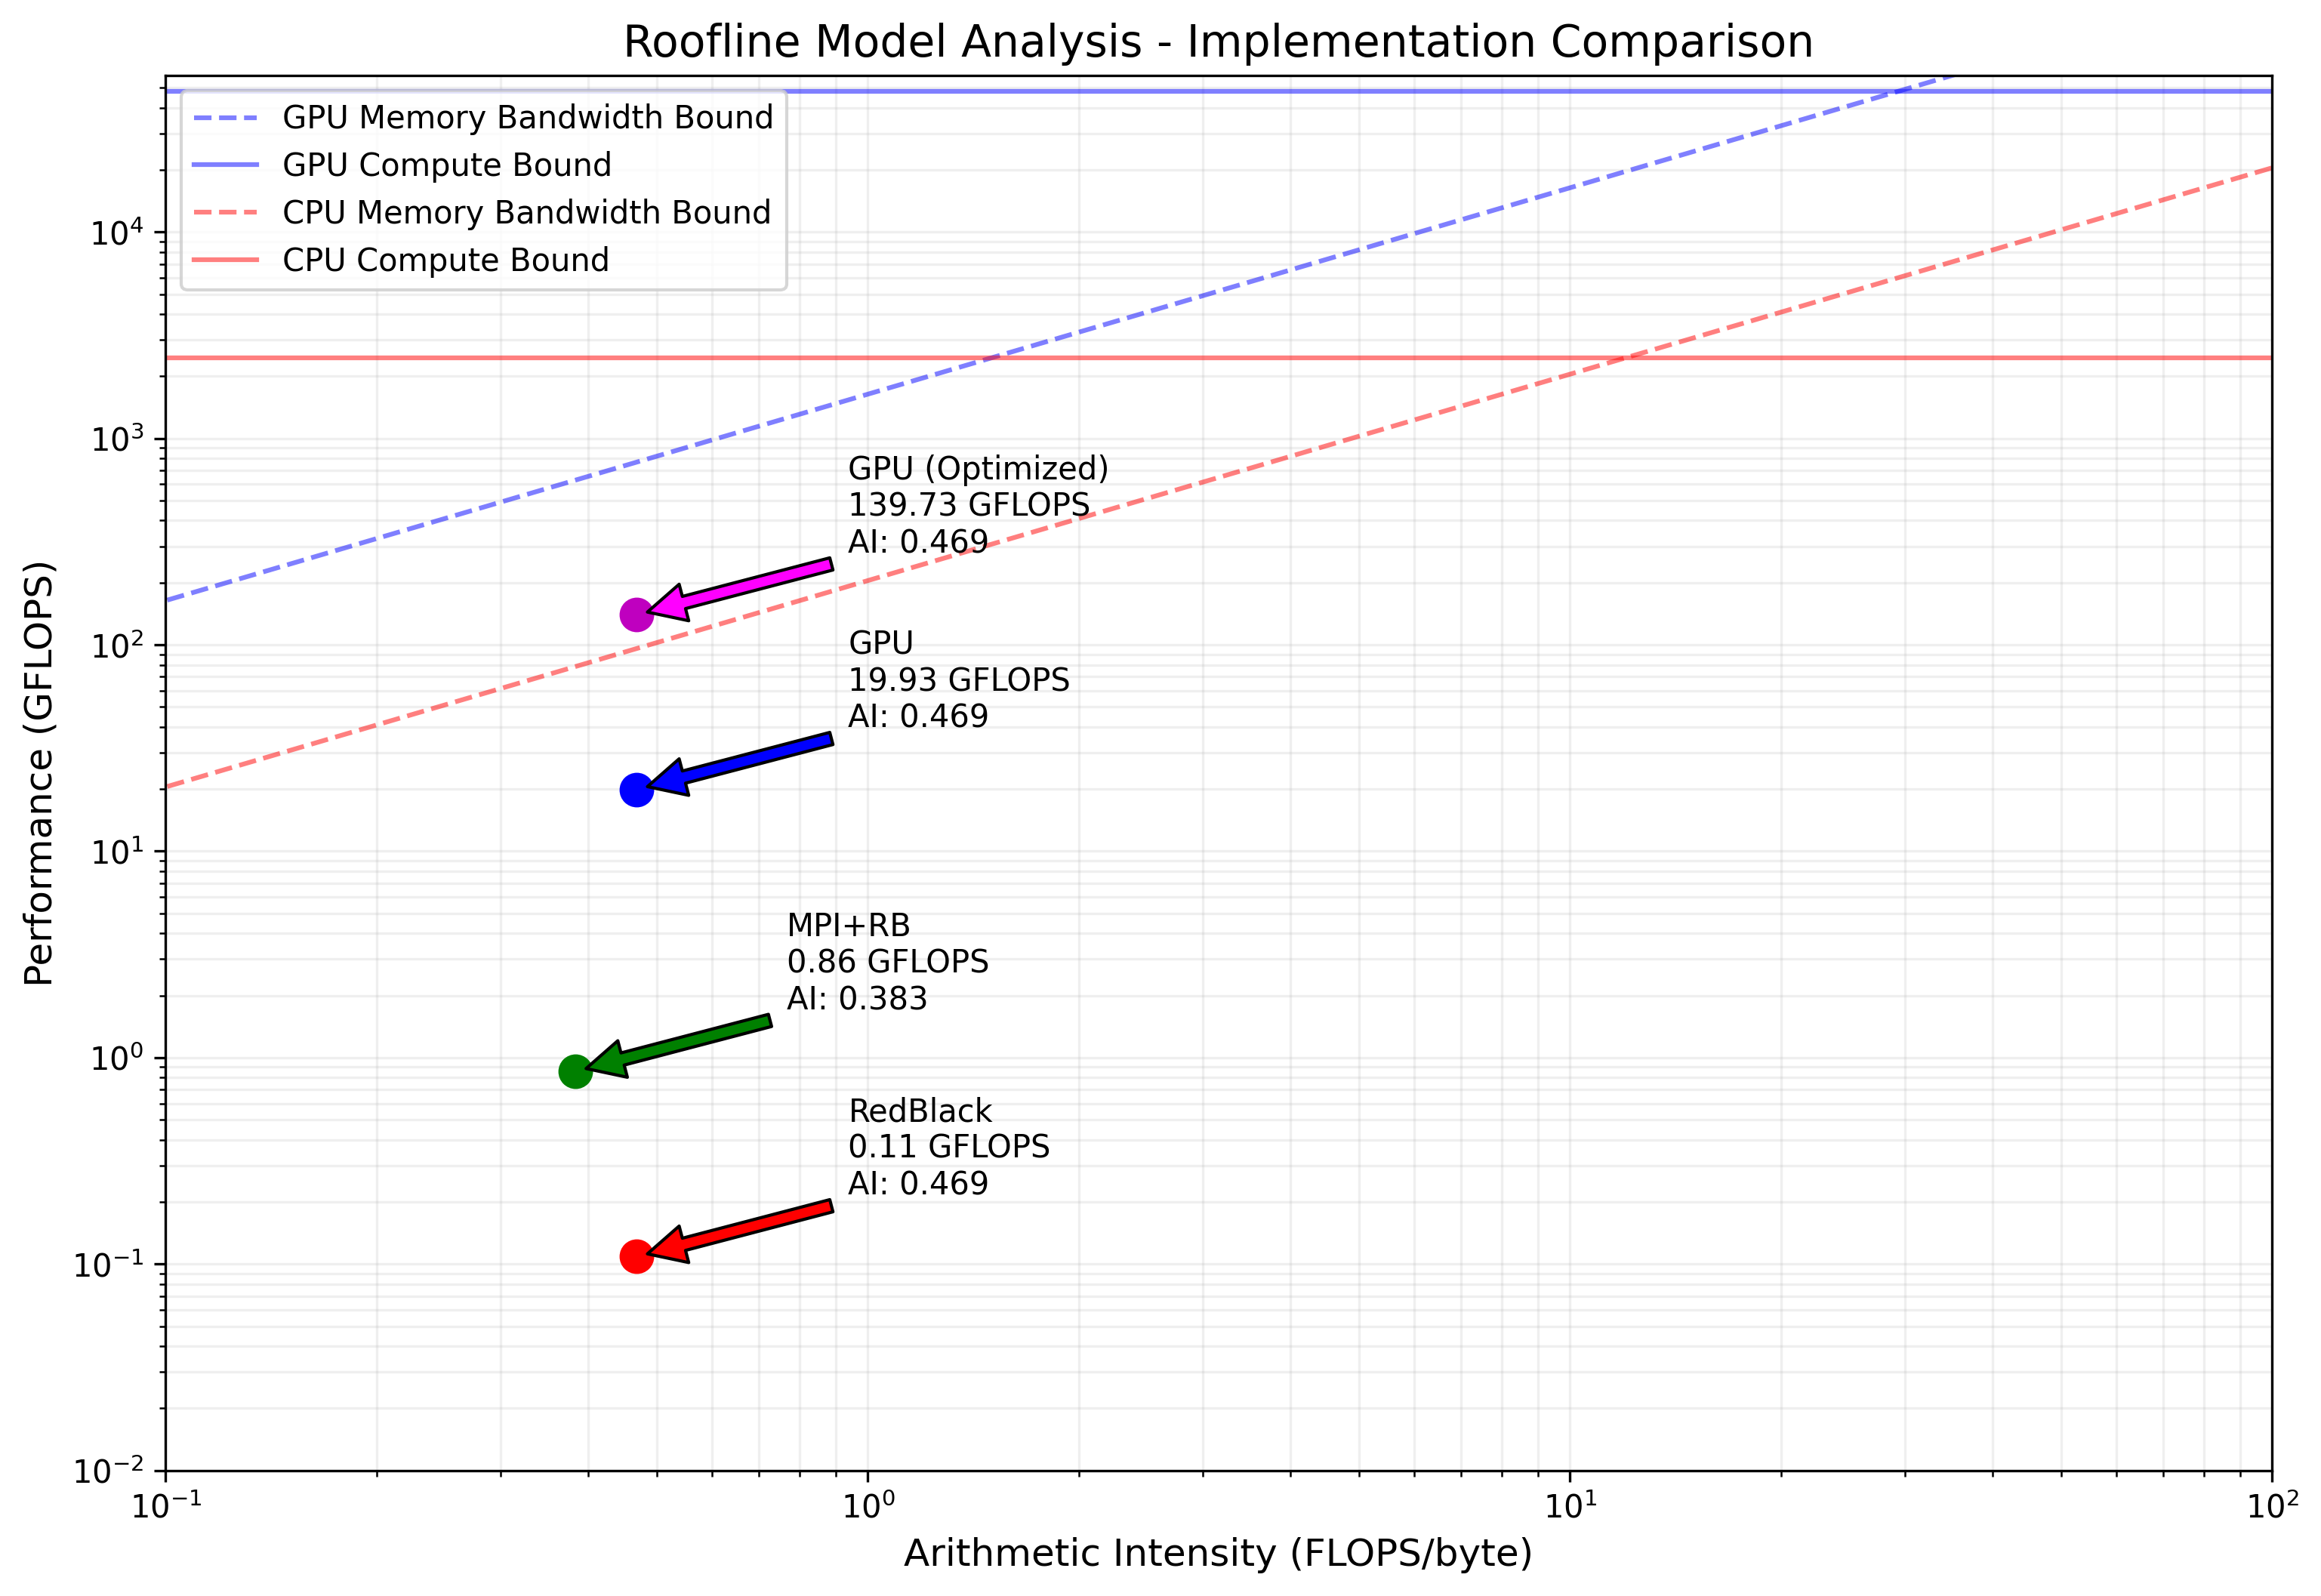
\includegraphics[width=\textwidth]{roofline_comparison.png}
\caption{Roofline model analysis comparing different implementations}
\label{fig:roofline}
\end{figure}

Our analysis reveals that all implementations are memory-bound, operating well below their respective ridge points (AMD MI250X GPU: 29.2 FLOPS/byte, AMD EPYC 7V13 CPU: 12.0 FLOPS/byte). This is expected given the nature of the Ising model computation, where each spin update requires reading multiple neighboring values but performs relatively few arithmetic operations.

The baseline GPU implementation achieves 19.93 GFLOPS with a memory bandwidth utilization of 42.52 GB/s. However, our optimized GPU implementation shows significant improvement, reaching 139.73 GFLOPS and 298.09 GB/s memory bandwidth, approximately a 7x performance increase. This improvement can be attributed to our optimizations in memory access patterns, particularly the use of shared memory and improved data locality.

The RedBlack CPU implementation operates at 0.11 GFLOPS with a memory bandwidth of 0.23 GB/s, while the MPI+RedBlack version achieves 0.86 GFLOPS and 2.24 GB/s memory bandwidth. Both CPU implementations show relatively low hardware utilization, suggesting potential for further optimization.

\subsection{Scalability}
Performance is evaluated across varying lattice sizes ($64^3$ and $256^3$). Looking at our results, we see our optimized GPU implementation take 0.28s for a lattice size of $64^3$ and 5.5s for a lattice size of $256^3$. 
While this is a 64x increase in lattice size, we only have a ~19.6x increase in runtime. This is a clear indication of our parallelization successfully scaling and improving at scale.

\subsection{Implementation Comparison}
Our performance analysis reveals significant differences between implementations:

\begin{itemize}
    \item \textbf{Serial vs. MPI}: The single-rank MPI implementation performs similarly to the serial version (36.2s vs 35.6s), but scaling to 8 ranks yields a near-linear speedup, reducing runtime to 5.8s. This demonstrates effective parallelization with minimal overhead.
    
    \item \textbf{CPU vs. GPU}: The baseline GPU implementation outperforms both serial and MPI versions significantly, completing the same workload in 0.95s. This represents a 38x speedup over serial and 6.1x over 8-rank MPI implementation.
    
    \item \textbf{Optimized GPU}: Our optimizations (shared memory, GPU-aware MPI, precomputed random numbers) further reduced the GPU runtime to 0.28s, achieving a 129x speedup over serial and a 3.4x improvement over the baseline GPU implementation.
    
    \item \textbf{Scaling Behavior}: When increasing the problem size from $64^3$ to $256^3$ (64x more lattice points), the optimized GPU implementation shows excellent scaling, with runtime increasing only by a factor of 19.6 (from 0.28s to 5.5s).
\end{itemize}

The efficiency analysis shows that our optimized GPU implementation achieves the highest hardware utilization, though still well below theoretical peaks due to the memory-bound nature of the algorithm. The MPI implementation demonstrates good scaling but is limited by the AMD EPYC 7V13 CPU memory bandwidth, while the GPU implementations benefit from the significantly higher memory bandwidth available on the AMD MI250X GPU accelerator.

\section{Results}
\subsection{Energy and Magnetization}
The energy and magnetization are plotted as functions of iteration count, demonstrating the convergence of the solution.
\begin{figure}[H]
\centering
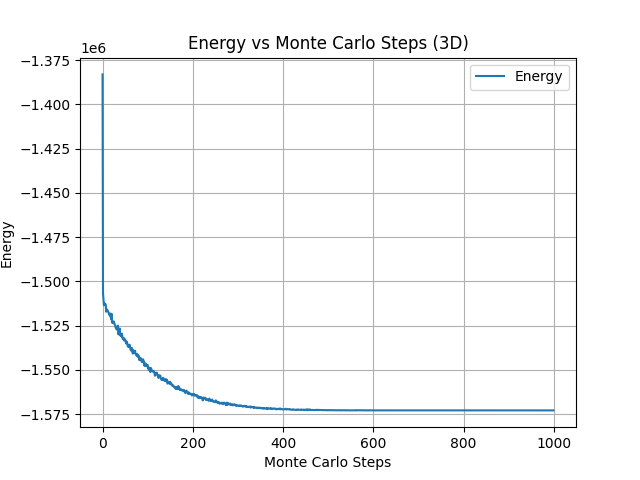
\includegraphics[width=0.7\textwidth]{energy_vs_steps.png}
\caption{Energy vs Iteration Count}
\label{fig:energy_vs_steps}
\end{figure}

\begin{figure}[H]
\centering
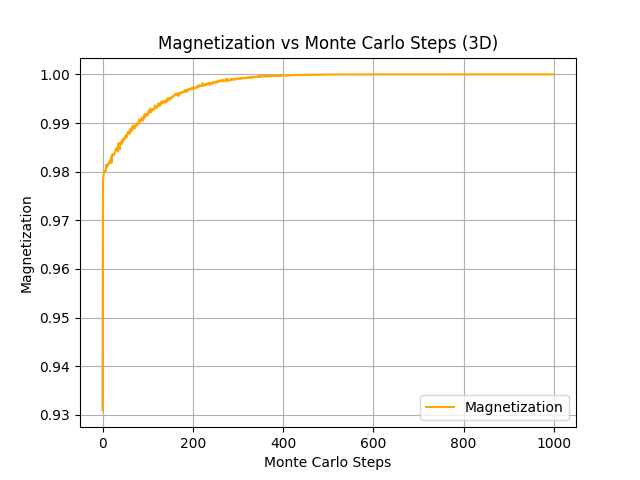
\includegraphics[width=0.7\textwidth]{magnetization_vs_steps.png}
\caption{Magnetization vs Iteration Count}
\label{fig:magnetization_vs_steps}
\end{figure}


\subsection{Visualization}
In addition to metadata, such as the energy and magnetization, we can also visualize the spins on the lattice. Figure~\ref{fig:spins} shows the spins on the lattice at a given iteration.

\begin{figure}[H]
\centering
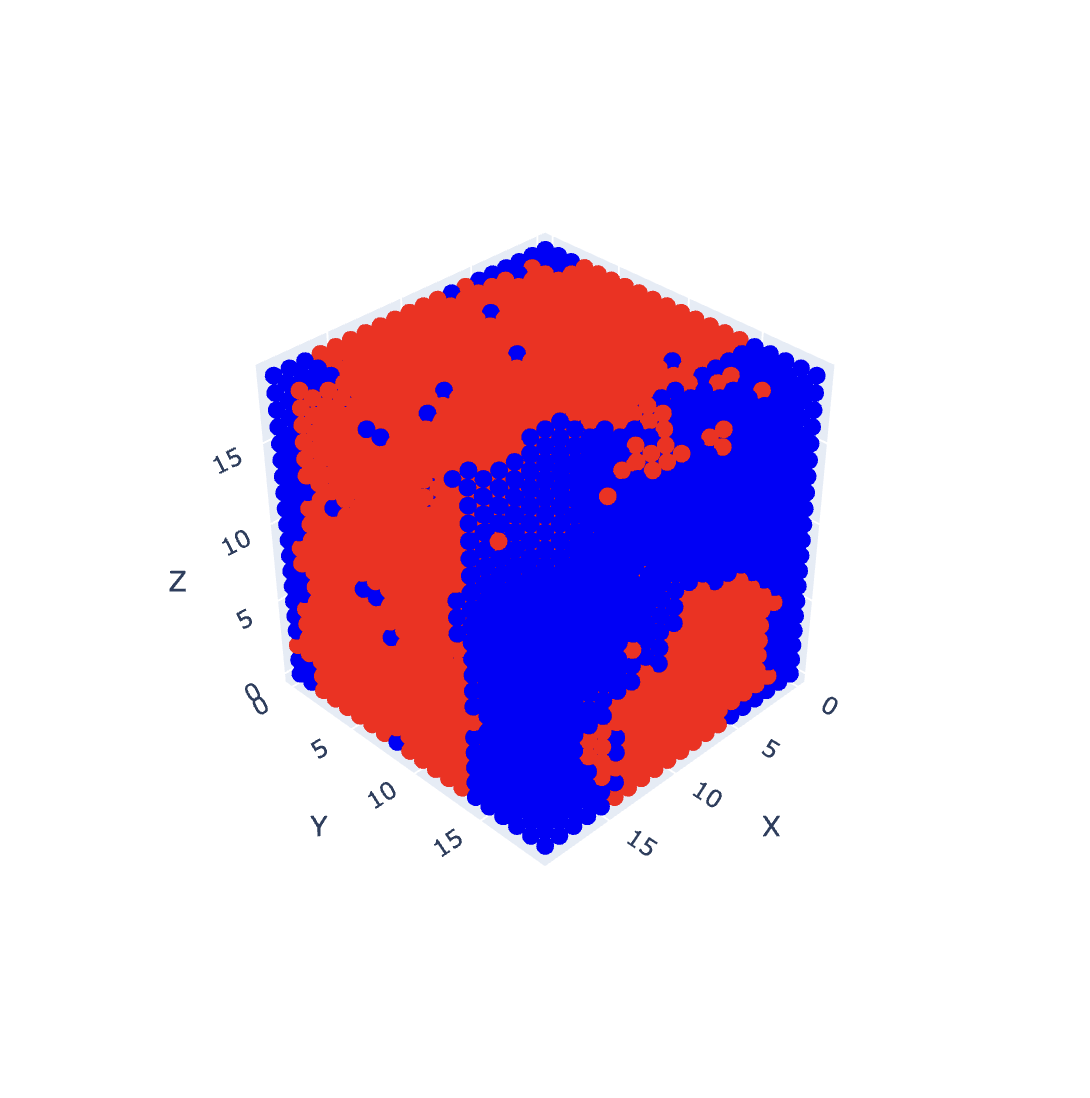
\includegraphics[width=0.7\textwidth]{lattice.png}
\caption{Spins on the Lattice}
\label{fig:spins}
\end{figure}

An interactive web demo can be found at \url{https://tajgillin.neocities.org/redblack/rb}.

\section{Discussion}
The implementation and analysis of the 3D Ising model reveals several key insights about parallel computing strategies and their effectiveness. Our results demonstrate that while both MPI and GPU implementations offer significant performance improvements over the serial version, the optimized GPU implementation provides the best performance, achieving a 129x speedup over the serial implementation.

The performance analysis highlights several important findings:

\begin{itemize}
    \item The red-black update scheme successfully prevents pattern formation and enables parallel updates, proving essential for both MPI and GPU implementations.
    
    \item Memory access patterns significantly impact performance, as shown by the substantial improvements achieved through shared memory optimizations and GPU-aware MPI.
    
    \item The roofline analysis reveals that all implementations are memory-bound, suggesting that future optimizations should focus on improving memory access patterns rather than computational efficiency.
    
    \item The excellent scaling behavior of our optimized GPU implementation (19.6x increase in runtime for a 64x increase in problem size) indicates effective parallelization and proper utilization of GPU resources.
\end{itemize}

While our implementation achieves significant speedup, the roofline analysis suggests we are still operating below theoretical hardware limits. This indicates potential for further optimization, particularly in memory access patterns and communication strategies. The proposed future enhancements, such as pinned memory and asynchronous streams, could help bridge this performance gap.

Briefly, from a physics perspective, I will mention we see the expected results. Notably, this simulation is being ran at low temperature, and we are seeing spontaneous polarization! At high temperatures, we simply see thermal fluctuations. The visual demo is quite fun to play with, and I encourage you to check it out if you can.

\section{Future Directions}
\subsection{Pinned Memory}
One promising avenue for optimization involves the implementation of pinned memory for GPU operations. Currently, our implementation uses pageable host memory for CPU-GPU transfers, which requires the CUDA driver to first copy the data to a temporary pinned buffer before transfer. By directly allocating pinned memory, we can eliminate this extra copy and achieve higher bandwidth for memory transfers. While pinned memory requires more careful memory management due to its limited availability, the potential performance benefits make it an attractive optimization target.


\subsection{Asynchronous Streams}
A significant optimization opportunity lies in the implementation of asynchronous CUDA streams to overlap computation and communication. The current implementation processes halo exchanges and core computations sequentially, leading to idle GPU resources during communication phases. By dividing the computation domain into interior and boundary regions, we could compute the interior while simultaneously performing halo exchanges for the boundaries. This approach would require careful stream synchronization but could significantly reduce the overall runtime by hiding communication latency behind useful computation. The implementation would involve launching separate kernels for interior and boundary regions, with boundary computations scheduled after their respective halo exchanges complete.

\subsection{Temperature Scaling}
From a physics perspective, extending the simulation to study temperature scaling effects would provide valuable insights into phase transitions. This would involve implementing an automated temperature sweep mechanism to observe the system's behavior around the critical temperature. Such an extension would require careful consideration of equilibration times at different temperatures and could benefit from adaptive step sizing near the critical point. This enhancement would not only improve the physical relevance of our simulation but also provide opportunities for additional performance optimizations specific to different temperature regimes.

\section{Conclusion}
This project has successfully demonstrated the implementation and optimization of a 3D Ising Model using modern high-performance computing techniques. Through careful application of parallel computing strategies, we achieved significant performance improvements, with our optimized GPU implementation delivering a 129x speedup over the serial version. The combination of MPI domain decomposition and GPU acceleration proved particularly effective, allowing us to simulate larger systems with reasonable computational overhead.

Our performance analysis revealed the critical role of memory access patterns in determining overall efficiency. The implementation of shared memory optimizations and GPU-aware MPI significantly reduced communication overhead, though the roofline analysis suggests potential for further improvements. The red-black update scheme proved essential for maintaining simulation accuracy while enabling parallel updates, demonstrating the importance of algorithm design in parallel implementations.

From a physics perspective, our implementation successfully captured the essential behavior of the 3D Ising model, including spontaneous magnetization at low temperatures and proper thermal fluctuations at higher temperatures. The interactive visualization tool provides an intuitive way to explore these phenomena, making the complex physics more accessible.

Looking forward, this work provides a foundation for future studies of more complex systems and optimization strategies. While we've achieved significant speedup, the identified optimization opportunities suggest exciting possibilities for even better performance in future implementations.


\newpage
\appendix
\section{Appendix}
Thanks for a great class Professor Grinberg!

\subsection{Pseudocode}

\subsubsection{GPU Implementation Details}
\begin{algorithm}[H]
\caption{GPU-Based Monte Carlo Implementation}
\begin{algorithmic}[1]
\State Create 3D MPI Cartesian communicator
\State Assign GPUs to MPI ranks (round-robin)
\State Allocate GPU memory for spins, energy, magnetization
\State Initialize cuRAND states for each lattice site
\For{each Monte Carlo step}
    \State // Red-Black Update Pattern with GPU Acceleration
    \For{color in \{red, black\}}
        \State Launch GPU kernel with 3D thread blocks (8x8x8)
        \For{each site of current color (parallel)}
            \State Calculate $\Delta E$ from 6 neighbors
            \State Generate random number using cuRAND
            \If{$\Delta E \leq 0$ or random $<$ $e^{-\Delta E/k_BT}$}
                \State Flip spin atomically
            \EndIf
        \EndFor
        \State Copy spins CPU $\leftrightarrow$ GPU
        \State Perform MPI halo exchange
        \State Copy updated halos CPU $\leftrightarrow$ GPU
    \EndFor
    \State // Energy Computation on GPU
    \State Launch reduction kernel with shared memory
    \State Compute local energy and magnetization
    \State MPI\_Reduce for global observables
    \If{time to save}
        \State Gather lattice to rank 0
        \State Write configuration to file
    \EndIf
\EndFor
\end{algorithmic}
\end{algorithm}

\begin{algorithm}[H]
\caption{GPU Energy Computation Kernel}
\begin{algorithmic}[1]
\State Allocate shared memory for block-level reduction
\For{each thread in parallel}
    \State Calculate site energy from 6 neighbors
    \State Store in shared memory
\EndFor
\State Synchronize threads
\For{reduction stride = block\_size/2 to 1}
    \If{thread\_id $<$ stride}
        \State Reduce energy values in shared memory
    \EndIf
    \State Synchronize threads
\EndFor
\If{thread\_id == 0}
    \State Atomic add block result to global counters
\EndIf
\end{algorithmic}
\end{algorithm}

\end{document}


